\documentclass[10pt]{beamer}
%Information to be included in the title page:
\title{Taller de Instalación de Linux}
\author{RoboTech URJC}
\institute{URJC}
\date{2023}
\usetheme{Madrid}
\usecolortheme{beaver}
\usepackage{graphicx} %LaTeX package to import graphics
\graphicspath{{images/}} %configuring the graphicx package
\logo{
\includegraphics[width=0.25\textwidth]{logo}
\includegraphics[scale=0.2]{robotech}}

\begin{document}
	
	\frame{\titlepage}
	
	\begin{frame}
		\frametitle{¿Quiénes somos?}
		\begin{itemize}			
			\item Alba Cruz Rodríguez: \\
			Estudiante de ingeniería robótica software (3º año).
			\item Iker Peral del Pino: \\
			Estudiante de ingeniería robótica software (3º año).
			\item Javier Izquierdo Hernández: \\
			Estudiante de ingeniería robótica software (3º año).
		\end{itemize}
		\vspace{20pt}
		\begin{center}
			
\includegraphics[width=15 pt]{twitter} \hspace{5 pt}
\includegraphics[width=15 pt]{instagram}\hspace{10 pt} @robotech\_urjc\\
			
			
\includegraphics[width=15 pt]{mail} \hspace{10 pt} robotechurjc@gmail.com
		\end{center}
	\end{frame}
	
	\begin{frame}
		\frametitle{Distribuciones de Linux}
		Muchas diferentes distribuciones para diferentes necesidades. La mayoría de ellas Open Source.\\
		\begin{center}
			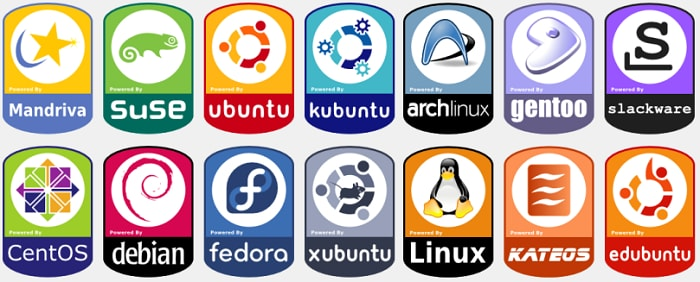
\includegraphics[width=0.5\textwidth]{linux_logo}
		\end{center}
	\end{frame}
	
	\begin{frame}
		\frametitle{¿Por qué Linux?}
		\begin{itemize}
			\item Linux es gratis.\\
			\item Mucho software es OpenSource.\\
			\item Infinidad de configuraciones diferentes.\\
			\item Más control sobre tu privacidad.\\
			\item Menos virus.\\
			\item Más sencillo programar en varios lenguages.
		\end{itemize}
	\end{frame}
	
	\begin{frame}
		\frametitle{Diferentes Escritorios. Sabores de Ubuntu}
		\begin{itemize}
			\item Gnome: Ubuntu estándar
			\item KDE: Tuxedo Os 2, Kubuntu
			\item Cinnamon: Mint, 
			Ubuntu Cinnamon
			\item Otros: Lubuntu, Ubuntu Budgie, 
			Ubuntu MATE ...
		\end{itemize}
	\end{frame}
	
	\begin{frame}
		\frametitle{Requisitos previos}
		\begin{itemize}
			\item Espacio disponible de al menos 50 Gb. Recomendado 150-200 Gb.
			\item  Usb de al meno 8 Gb vacio.
		\end{itemize}
	\end{frame}
	
	\begin{frame}
		\frametitle{Instalar Ubuntu desde Windows}
		Descargar Ubuntu 22.04 LTS .iso: https://ubuntu.com/download/desktop\\
		\begin{center}
			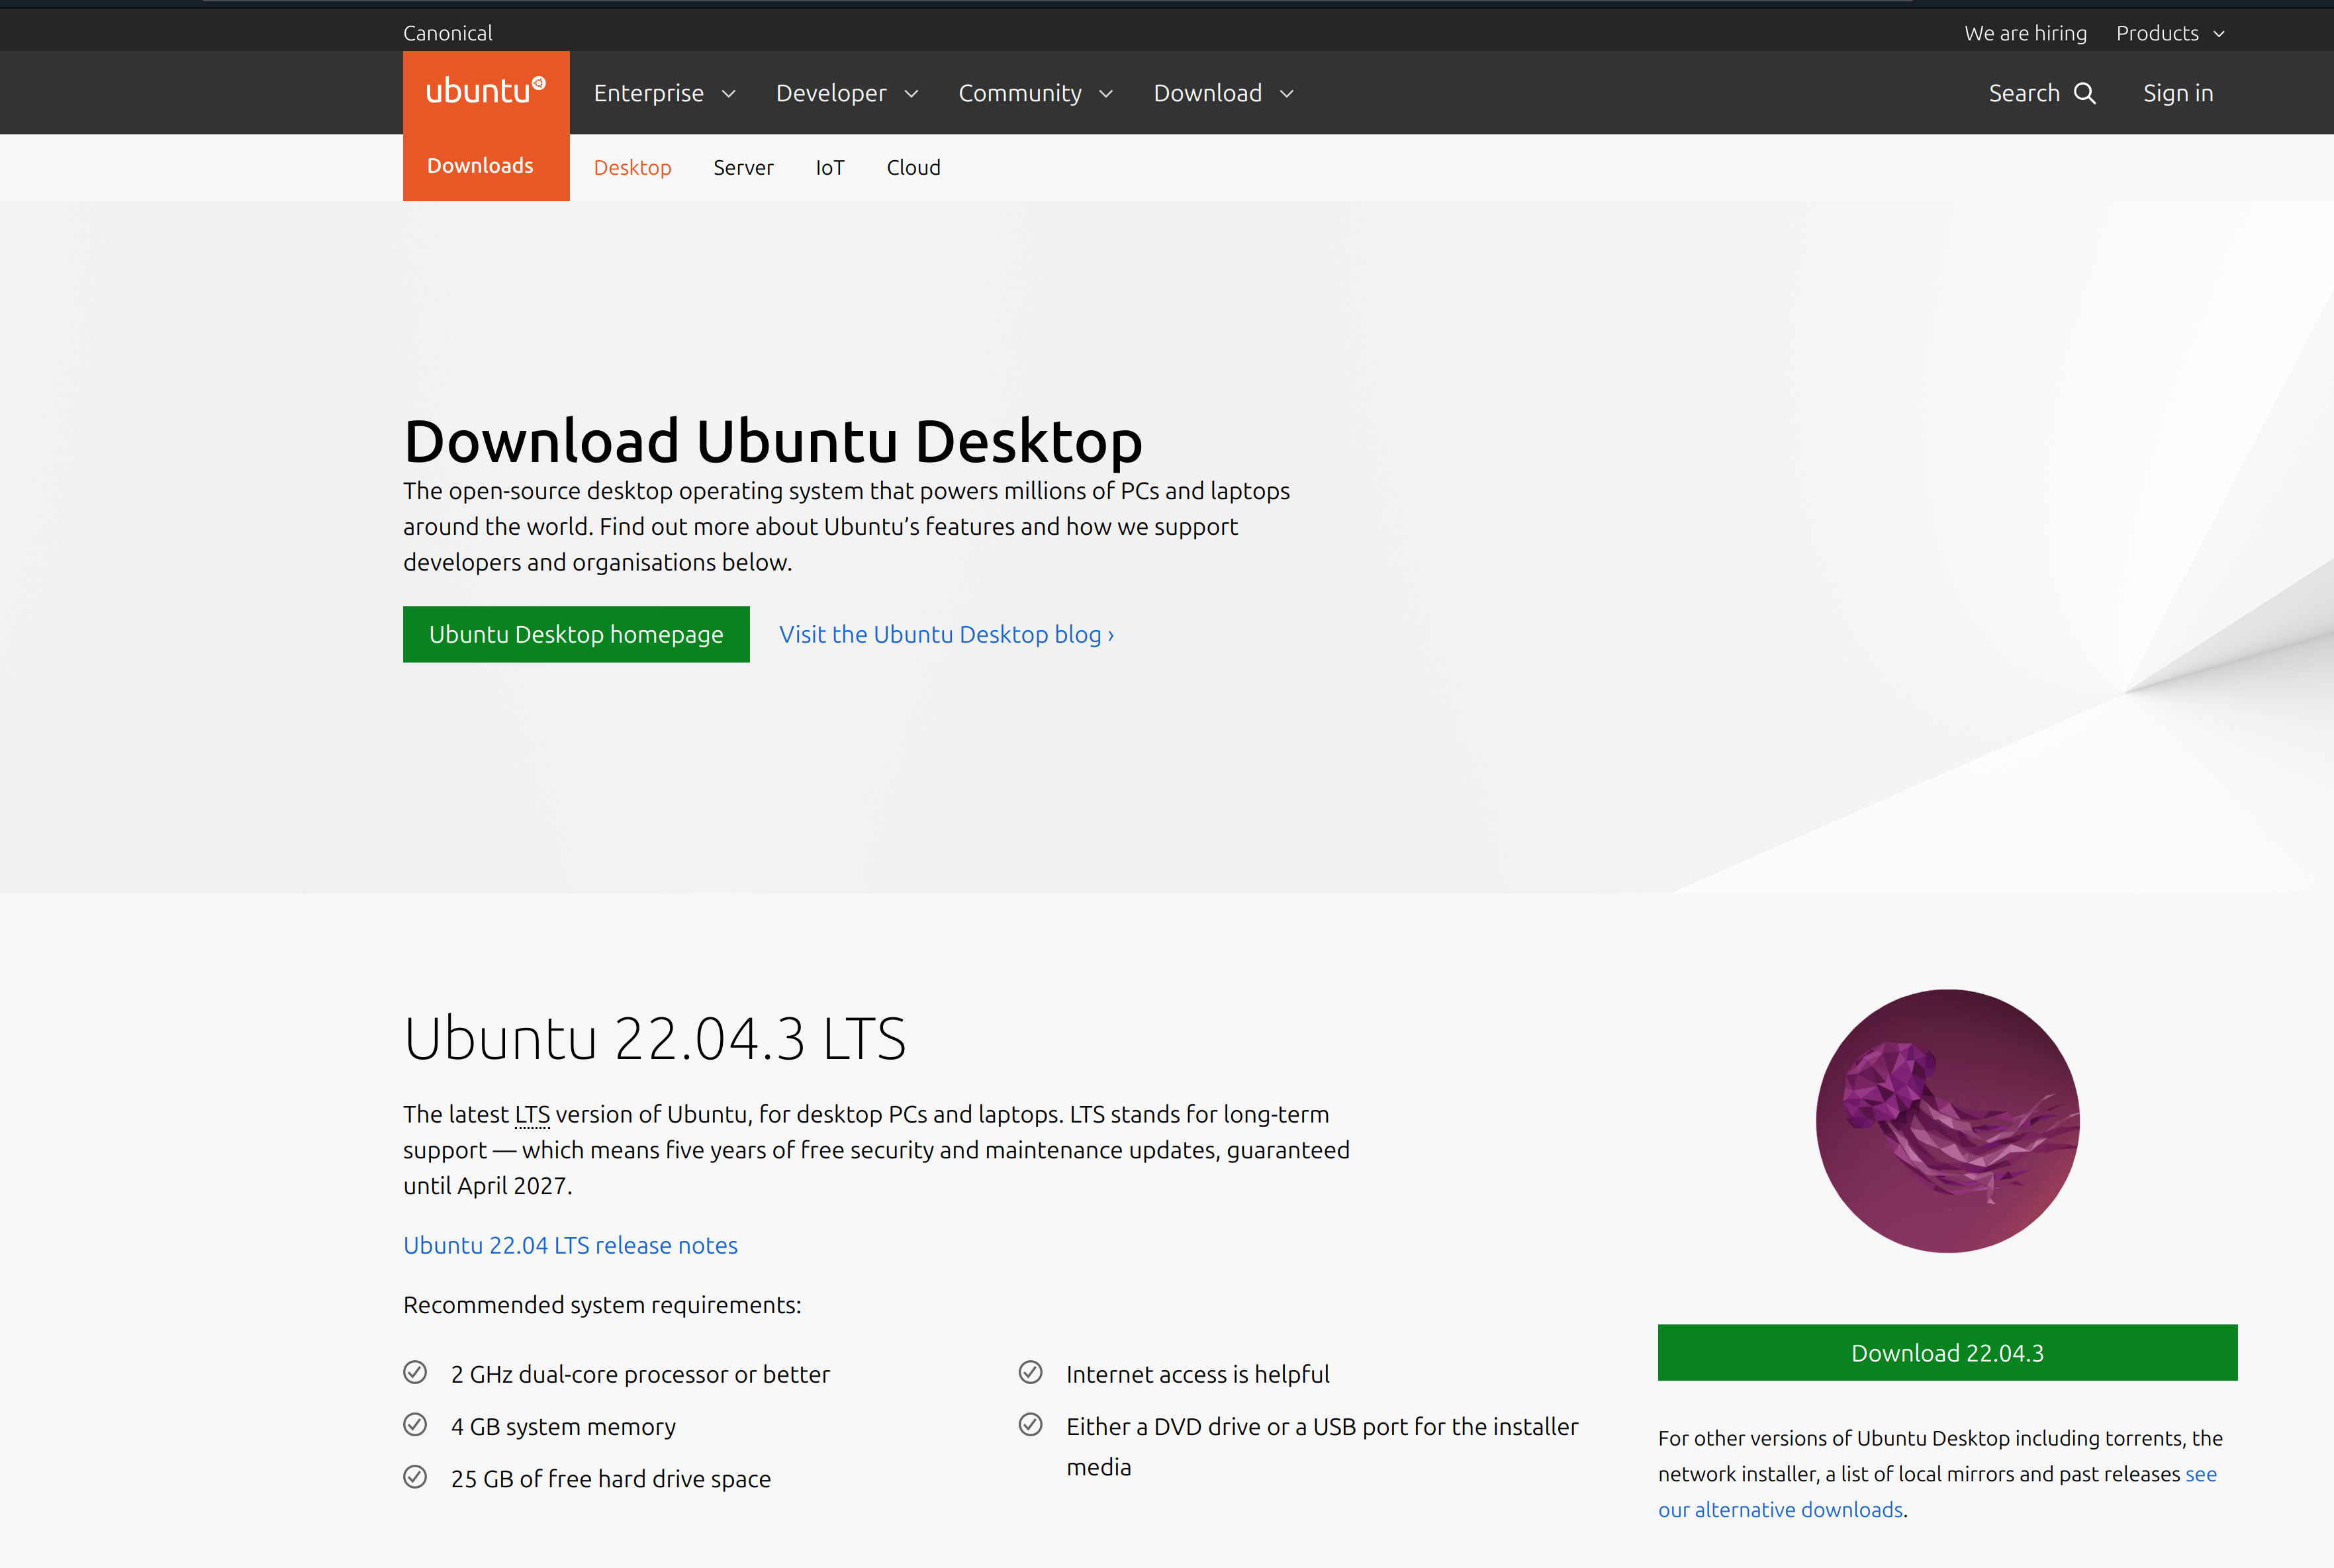
\includegraphics[width=0.5\textwidth]{ubuntu}
		\end{center}
	\end{frame}
	
	\begin{frame}
		\frametitle{Crear un USB Live en Windows}
		Instalar BalenaEtcher: https://etcher.balena.io\\
		\begin{itemize}
			\item Select image → El .iso descargado
			\item Select drive → El usb que vamos a usar para la instalación (mínimo 8gb)
			\item Flash!
		\end{itemize}
		\begin{center}
			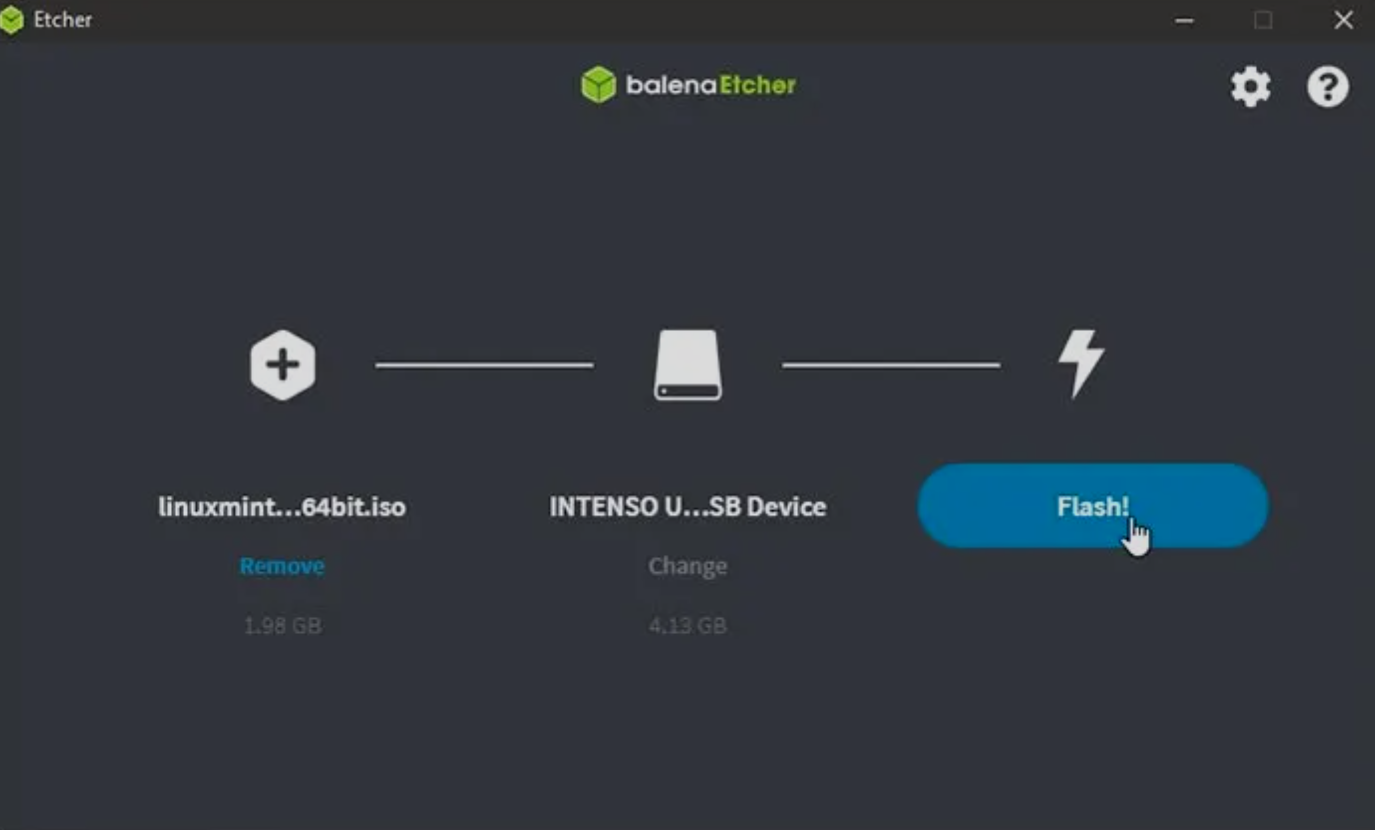
\includegraphics[width=0.5\textwidth]{balena}
		\end{center}
	\end{frame}
	
	\begin{frame}
		\frametitle{Iniciar Ubuntu}
		\begin{enumerate}
			\item Apagar el ordenador.
			\item Mientras encendemos el ordenador pulsamos F2 o F7 (puede ser otra tecla, depende del fabricante) para acceder a la BIOS o al boot menu.
			\item Seleccionamos arrancar desde el USB
		\end{enumerate}
	\end{frame}
	
	\begin{frame}
		\frametitle{Iniciar Ubuntu}
		Seleccionar \textbf{Install Ubuntu}. Si tienes NVIDIA a lo mejor tienes que seleccionar \textbf{(safe graphics)}.\\
		\begin{center}
			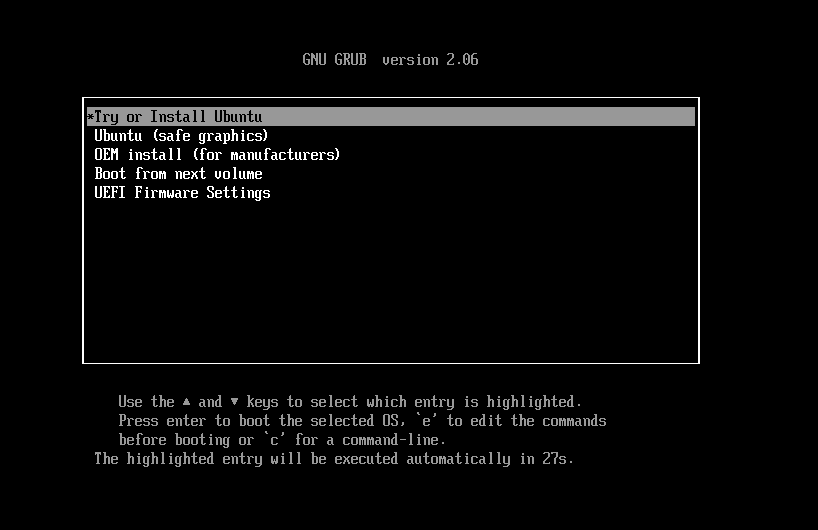
\includegraphics[width=0.5\textwidth]{install}
		\end{center}
	\end{frame}
	
	\begin{frame}
		\frametitle{Instalar Ubuntu}
		Seleccionar \textbf{Install Ubuntu} otra vez y dejarlo en \textbf{Inglés} o en \textbf{Español.} Recomendamos en Inglés.\\
		\begin{center}
			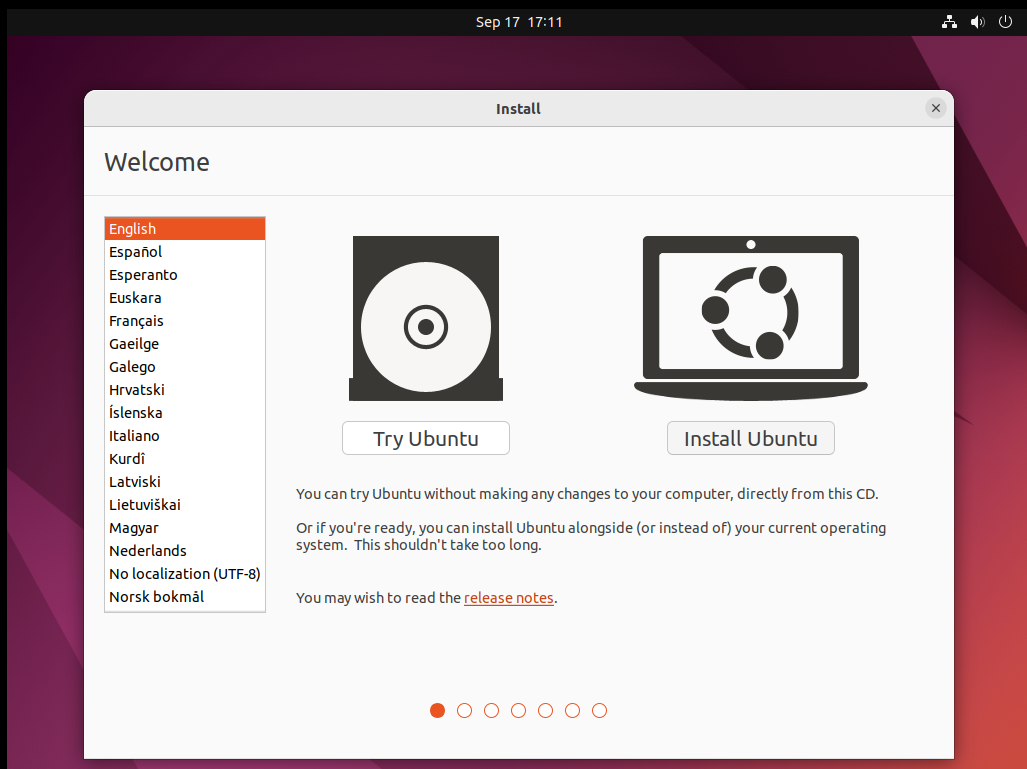
\includegraphics[width=0.5\textwidth]{install2}
		\end{center}
	\end{frame}
	
	\begin{frame}
		\frametitle{Instalar Ubuntu}
		Seleccionar el tipo de instalación. Recomendamos la instalación normal.\\
		Seleccionar la opción de third-party software.\\
		
		
		\begin{center}
			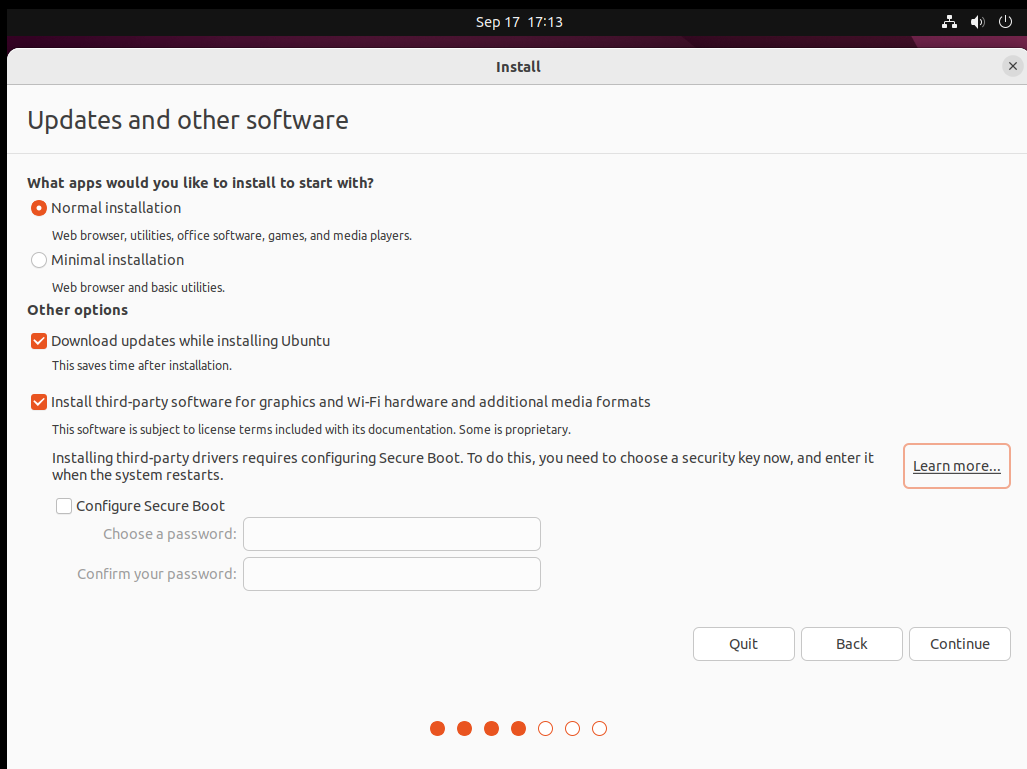
\includegraphics[width=0.5\textwidth]{installation}
		\end{center}
	\end{frame}
	
	\begin{frame}
		\frametitle{Instalar Ubuntu}
		Seleccionar el teclado correcto. Si no sabes cual es da en \textbf{Detect Keyboard Layout}.\\
		
		
		\begin{center}
			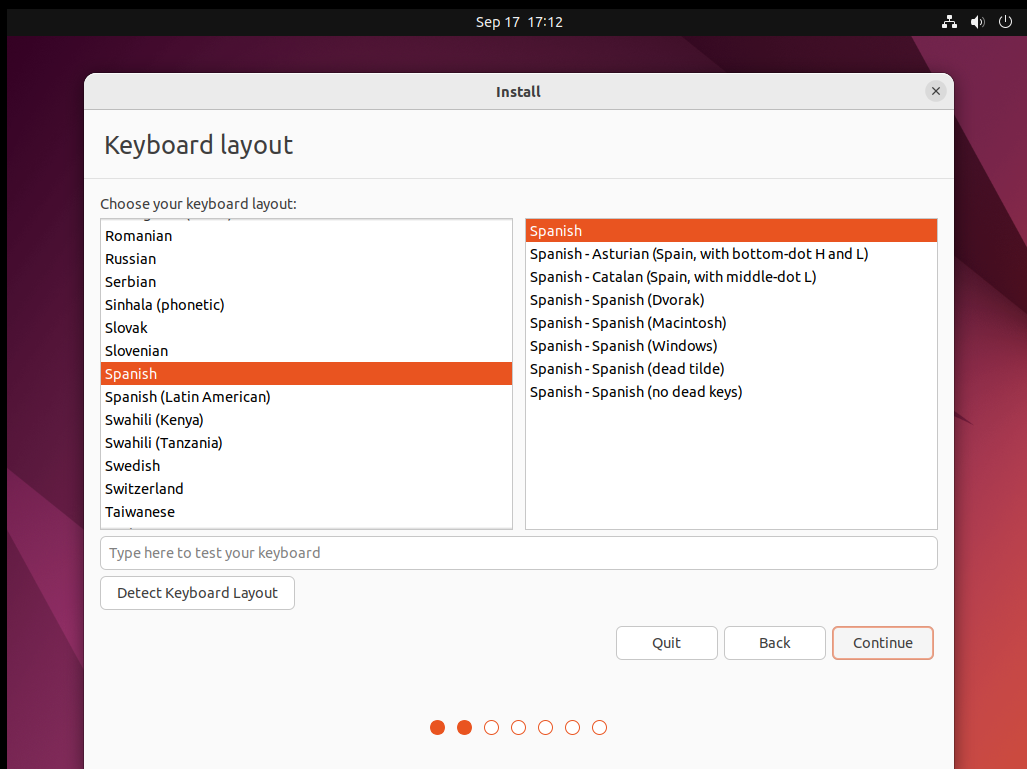
\includegraphics[width=0.5\textwidth]{keyboard}
		\end{center}
	\end{frame}
	
	\begin{frame}
		\frametitle{Instalar Ubuntu con Windows 10/11}
		\begin{alertblock}{Cuidado, no dudes en Preguntar}
			Seleccionar \textbf{Instalar junto con Windows 10/11}.
		\end{alertblock}
		
		\begin{center}
			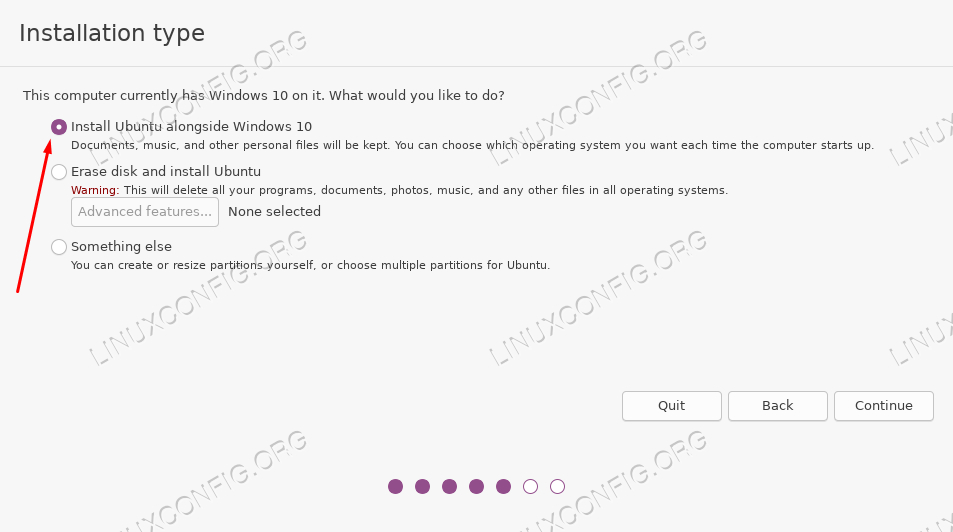
\includegraphics[width=0.5\textwidth]{windows-10}
		\end{center}
	\end{frame}
	
	\begin{frame}
		\frametitle{Instalar Ubuntu con Windows 10/11}
		\begin{alertblock}{Cuidado, no dudes en Preguntar}
			Mueve el slider de Ubuntu hasta un tamaño adecuado. Recomendado 150-200 Gb.
		\end{alertblock}
		
		\begin{center}
			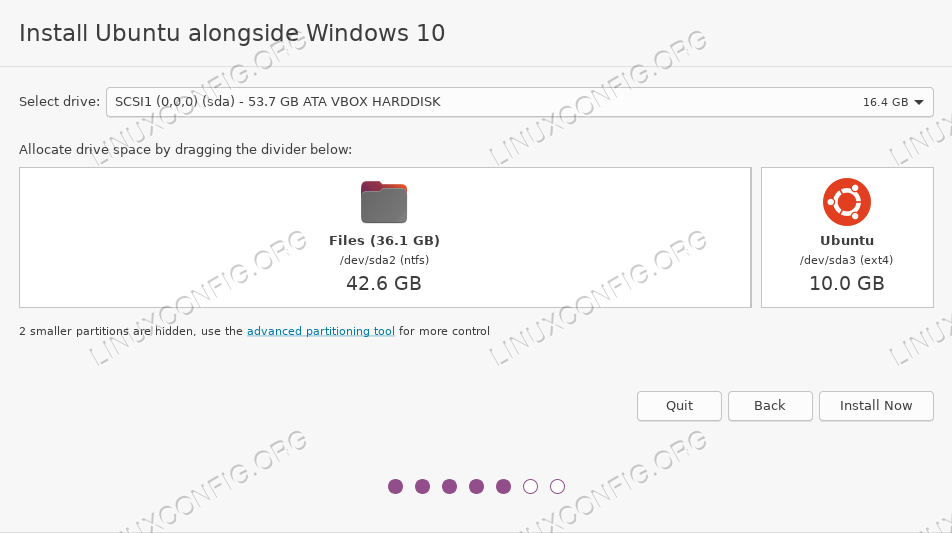
\includegraphics[width=0.5\textwidth]{windows-10-2}
		\end{center}
	\end{frame}
	
	\begin{frame}
		\frametitle{Instalar Ubuntu con Windows 10/11}
		\begin{alertblock}{Cuidado, no dudes en Preguntar}
			Acepta todos los avisos, sabiendo que lo que se borre será irreversible.
		\end{alertblock}
		
		\begin{center}
			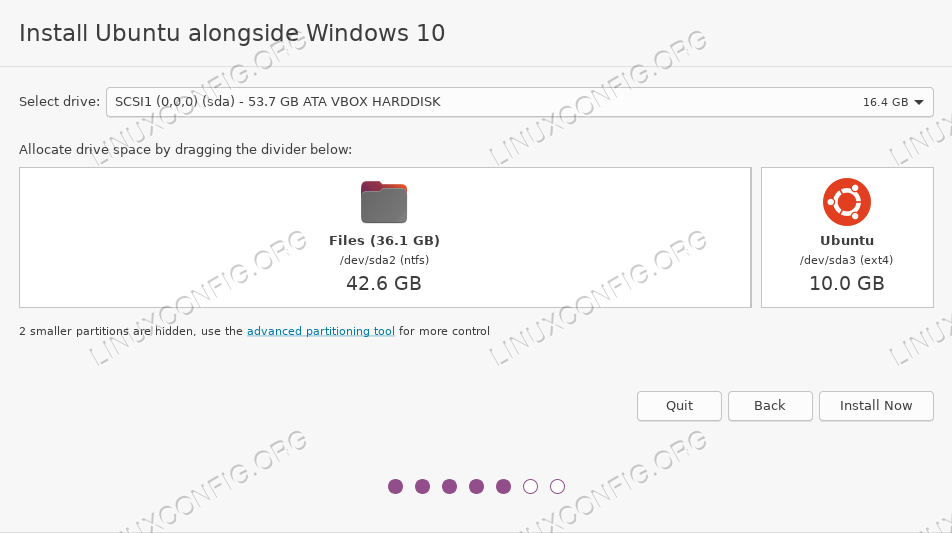
\includegraphics[width=0.5\textwidth]{windows-10-2}
		\end{center}
	\end{frame}
	
	\begin{frame}
		\frametitle{Acabar de Instalar Ubuntu}
		Selecciona la zona horaria de Madrid (Suele venir por defecto)
		.
		\begin{center}
			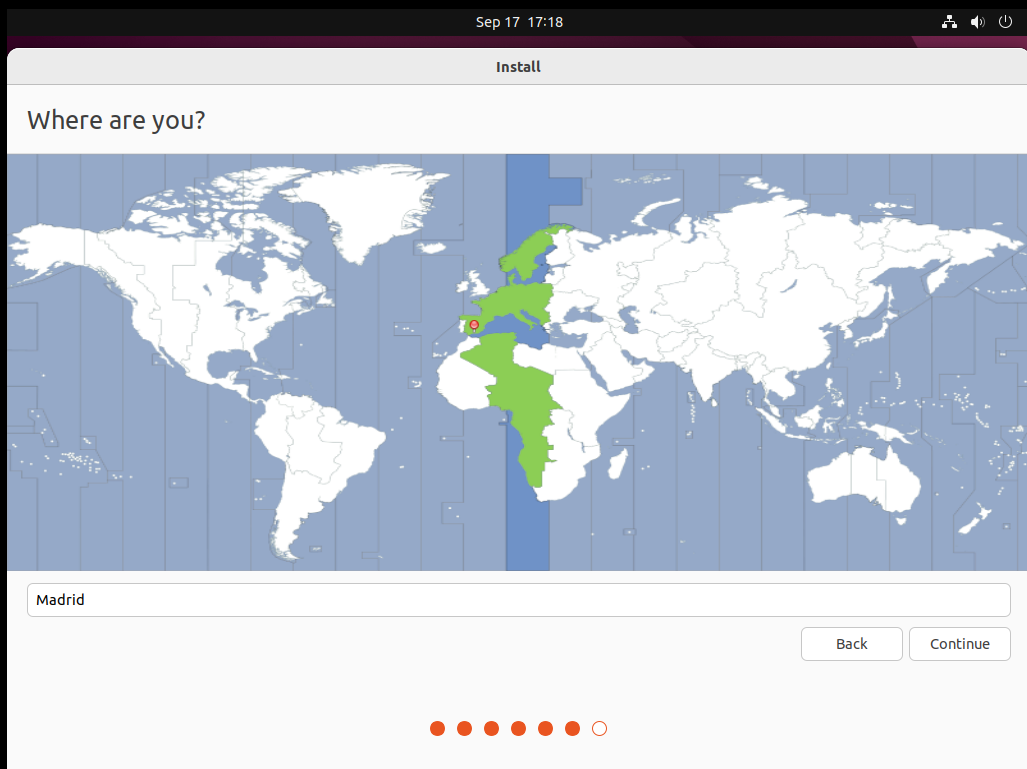
\includegraphics[width=0.5\textwidth]{timezone}
		\end{center}
	\end{frame}
	
	\begin{frame}
		\frametitle{Acabar de Instalar Ubuntu}
		Crea tu nombre y nombre de usuario. Luego rellena la contraseña.
		\begin{center}
			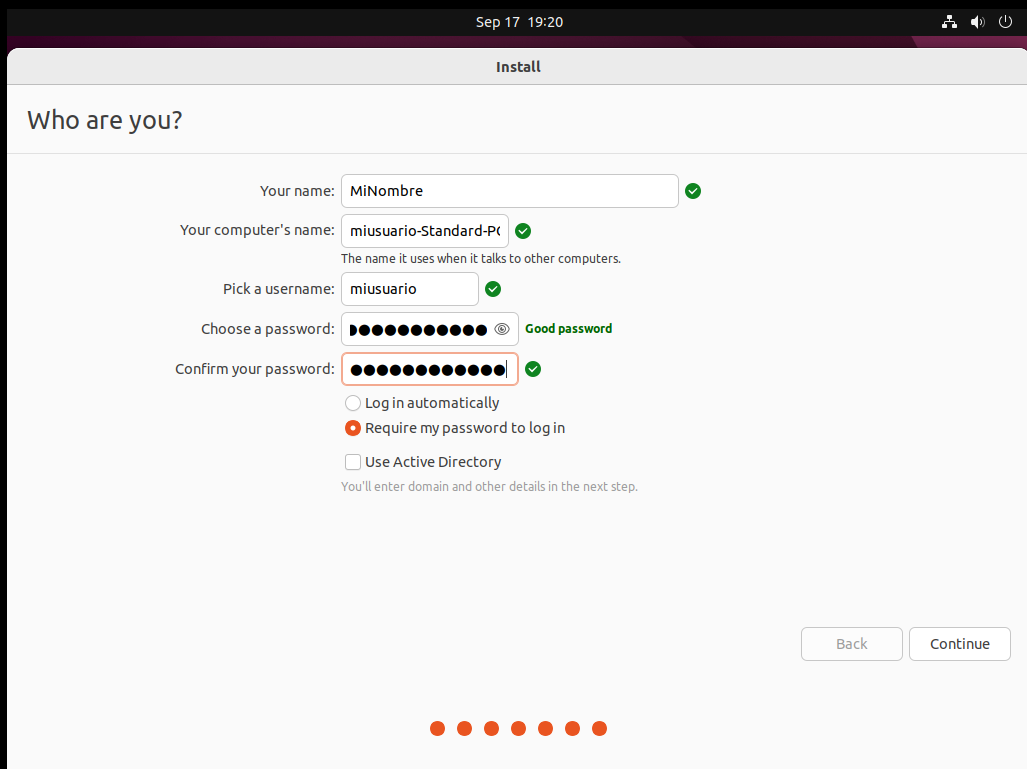
\includegraphics[width=0.5\textwidth]{login}
		\end{center}
	\end{frame}
	
	\begin{frame}
		\frametitle{Reinicia Ubuntu}
		Cuando este todo instalado te pedirá reiniciar el sistema.
		\begin{center}
			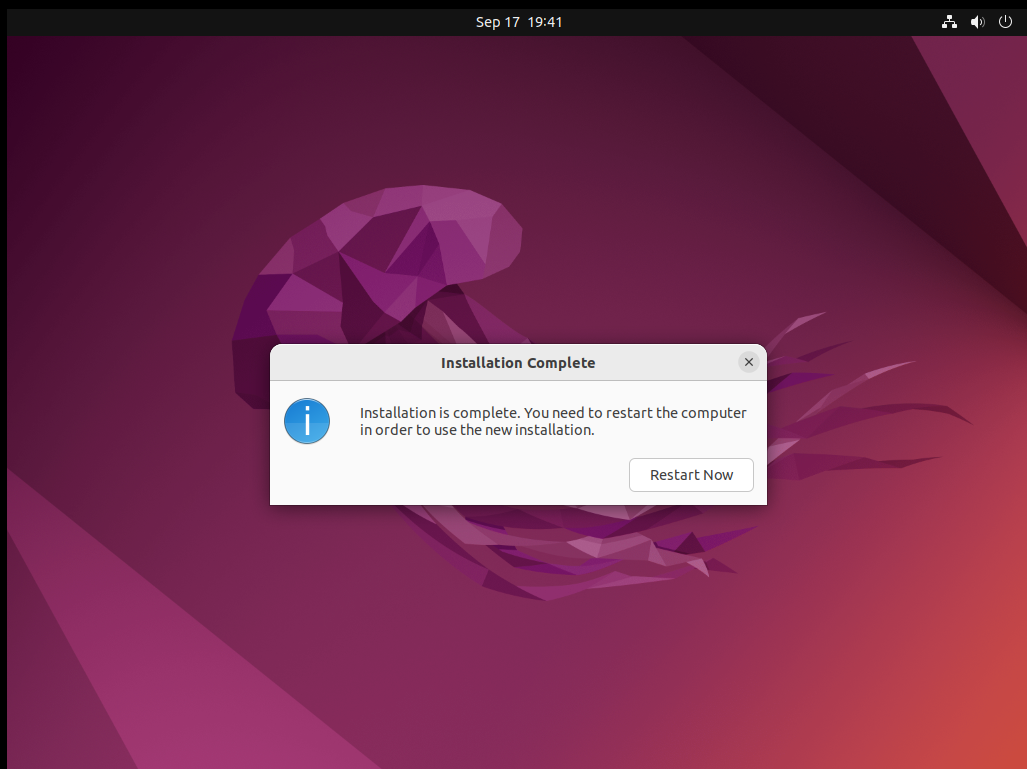
\includegraphics[width=0.5\textwidth]{restart}
		\end{center}
	\end{frame}
	
	\begin{frame}
		\frametitle{Algunos enlaces interesantes}
		\begin{itemize}
			\item GNU → https://www.gnu.org/
			\item FSF → https://www.fsf.org/
			\item Un blog de Open Source → https://itsfoss.com/
			\item Un canal de cosas relacionadas con linux → https://www.youtube.com/@TheLinuxEXP
		\end{itemize}
	\end{frame}

\end{document}